\documentclass[tikz]{standalone}

\begin{document}

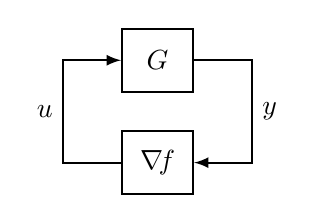
\begin{tikzpicture}[thick,>=latex,auto]
  \tikzstyle{block}=[draw,rectangle,inner sep=2mm,minimum width=0.9cm,minimum height=0.8cm]
  \def\dx{1.2}	% width of u,y loops
  \def\dy{1.3}	% v-dist of G and phi blocks
  \def\dk{0.9}	% separation of Psi attachments
  \node[block] (G) at (0,0) {$G$};
  \path (G) + (\dk,0) coordinate (yy);
  \path (G) + (-\dk,0) coordinate (uu);
  \node[block] (phi) at (0,-\dy) {$\nabla\!f$};
  \path (phi) + (\dk,0) coordinate (yy);
  \path (phi) + (-\dk,0) coordinate (uu);
  \draw[->] (phi) -- +(-\dx,0) |- node[pos=.25]{$u$} (G);
  \draw[<-] (phi) -- +(\dx,0) |- node[swap,pos=.25]{$y$} (G);
\end{tikzpicture}

\end{document}